\documentclass[../Interim_Report_Master]{subfiles}
\begin{document}
\hypertarget{fluid_mod}{\section{Fluid Model}\label{fluid_mod}}
As noted in the Literature Review the Lagrangian droplet model is normally coupled with a CFD code. Quite complex models could be used for this, for example, for investigations into the effect of turbulence. However, the focus here is getting a droplet evaporation model to be solved on a GPU and to investigate some statistics. Complex CFD codes could be added at a later date.

\subsection{Taylor-Green Vortex}
A set of analytic expressions for the fluid velocity will be used. The previous IP used a Taylor-Green vortex and that is what will also be used here. It is defined as:
\begin{subequations}
\begin{align}
U &= A\cos\left(a\left(x+\frac{\pi}{2a}\right)\right) \sin\left(a\left(y+\frac{\pi}{2a}\right)\right) \cos\left(a\left(z+\frac{\pi}{2a}\right)\right) \\
V &= A\sin\left(a\left(x+\frac{\pi}{2a}\right)\right) \cos\left(a\left(y+\frac{\pi}{2a}\right)\right) \sin\left(a\left(z+\frac{\pi}{2a}\right)\right) \\
W &= -2A\sin\left(a\left(x+\frac{\pi}{2a}\right)\right) \sin\left(a\left(y+\frac{\pi}{2a}\right)\right) \cos\left(a\left(z+\frac{\pi}{2a}\right)\right)
\end{align}
\end{subequations}

With $A$ defined as the flow magnitude and $a$ defined as the vortex frequency. This flow field is visualised in Figure \ref{tgv_plot}.
\begin{figure}
	\centering
	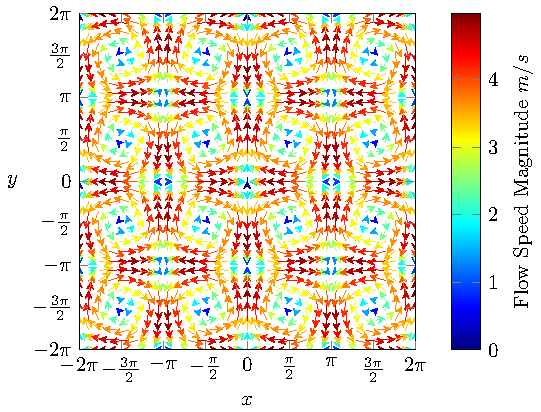
\includegraphics[width=0.8\textwidth]{./Diagrams/taylor_green_vortex.pdf}
	\caption{A 2D $xy$ vector field of a Taylor-Green vortex. Using $A=5$, $a=1$ and a domain length of $4\pi$.}
	\label{tgv_plot}
\end{figure}

The length of one of the individual vortices is the characteristic length $l_0$ used in defining the Stokes number.
\begin{equation}
Stk = \frac{\tau_{d0} u_0}{l_0}
\end{equation}

Where:
\begin{subequations}
\begin{align}
\tau_{d0} &= \frac{\rho_d D^2}{18\mu_G} \\
u_0 &= 0.7839A \\
l_0 &= \frac{\pi}{a} 
\end{align}
\end{subequations}
In this case $l_0=\pi$ and $u_0=3.9195$  \cite{Elijah_GPU_Report}. The usage of the Stokes number can be found in Section \ref{stat_test_case}.
\end{document}